%!TEX root = ../NCVC4.tex

\mysection{上下異形状切削}

\subsection{上下異形状切削用のCAD作図}
 図\ref{fig:sample1.pdf} とほぼ同じですが,切削レイヤを2つに分けてみます.
レイヤ名は名前順に並び替えられますので,大きい方の図形があとにくるレイヤ名に設定しましょう.
つまりXY軸(下側)の動きをCAM1に,UV軸(上側)の動きをCAM2に作図します.
抜け落ちても良いなら逆でもOKです.

\begin{figure}[H]
\centering
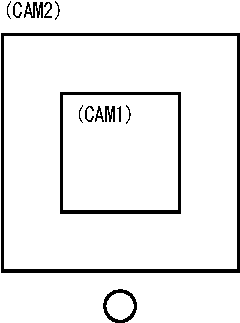
\includegraphics{No2/fig/sample2-crop.pdf}
\caption{上下異形状切削用のサンプル図形1}
\label{fig:sample2.pdf}
\end{figure}

 もうだいたい想像できると思いますが,切削レイヤを2つに分けると自動的に上下異形状切削のデータが出力されます.
基本的に上下の図形オブジェクト数を合わせれば,簡単に生成可能です.

\begin{figure}[H]
\centering
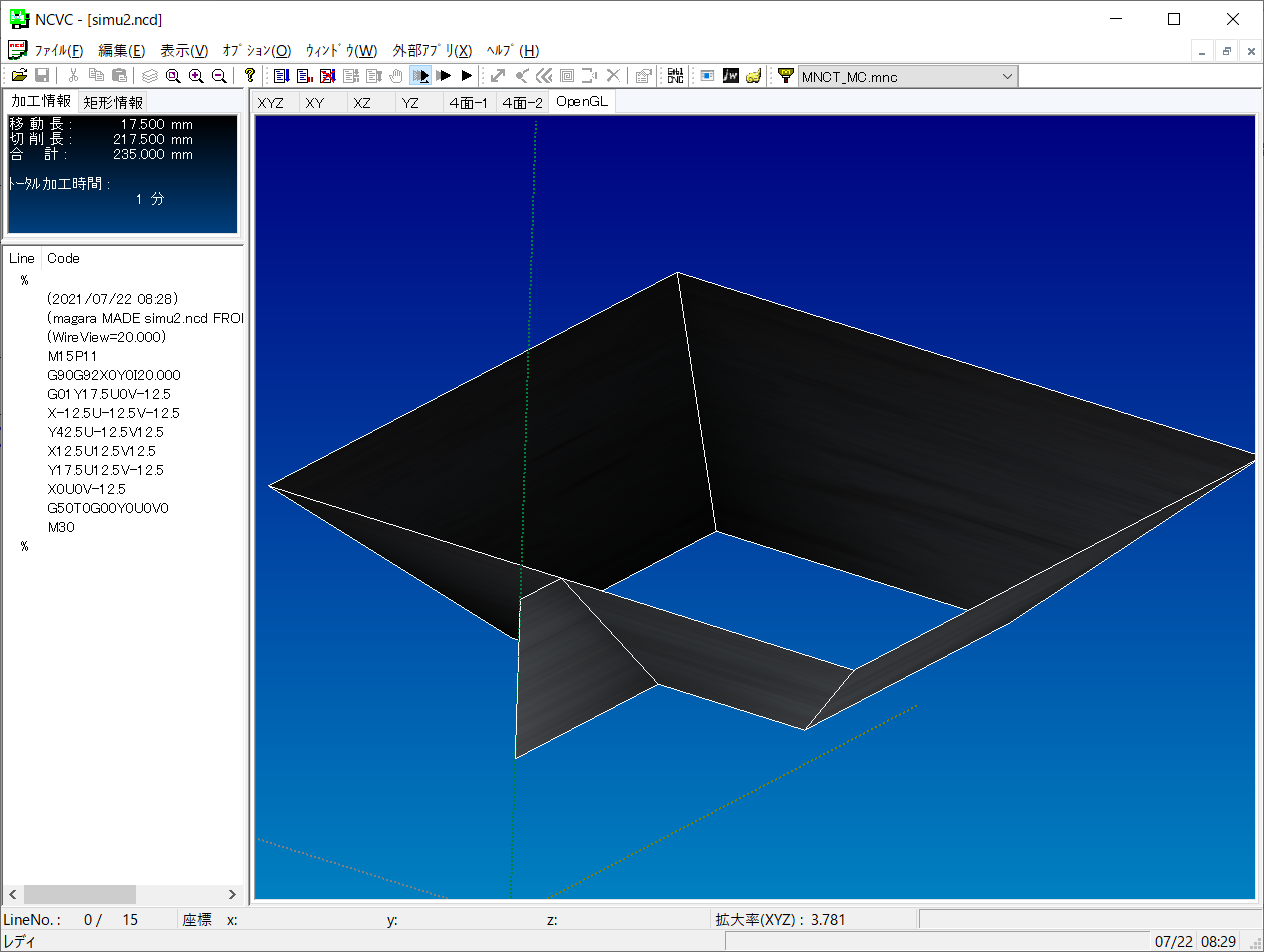
\includegraphics[scale=0.5]{No2/fig/simu2.png}
\caption{上下異形状切削のシミュレーション結果1}
\label{fig:simu2.png}
\end{figure}

 ただし,CAM1,CAM2ともに同じ方向へ動く必要があるため,形状認識処理からの方向指示で明確に切削方向を指示しておいてください.
それと,テーパ角度指示による上下異形状ではなくプログラム指示での上下異形状なので,テーパモードの指示を正しく設定しておきましょう.

\subsection{上下で図形の数が違う場合 その1}
 例えばXY軸が円でUV軸が四角形など,本当の意味で上下の形が違う(図形オブジェクトの数が違う)場合でも生成可能です.

\begin{figure}[H]
\centering
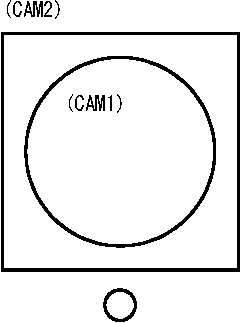
\includegraphics{No2/fig/sample3-crop.pdf}
\caption{上下異形状切削用のサンプル図形2}
\label{fig:sample3.pdf}
\end{figure}

 シミュレーション結果をワイヤフレームで見てみましょう.
図\ref{fig:simu3.png} のように微細線分の連続が生成され,望みの図形が切削されます.

\begin{figure}[H]
\centering
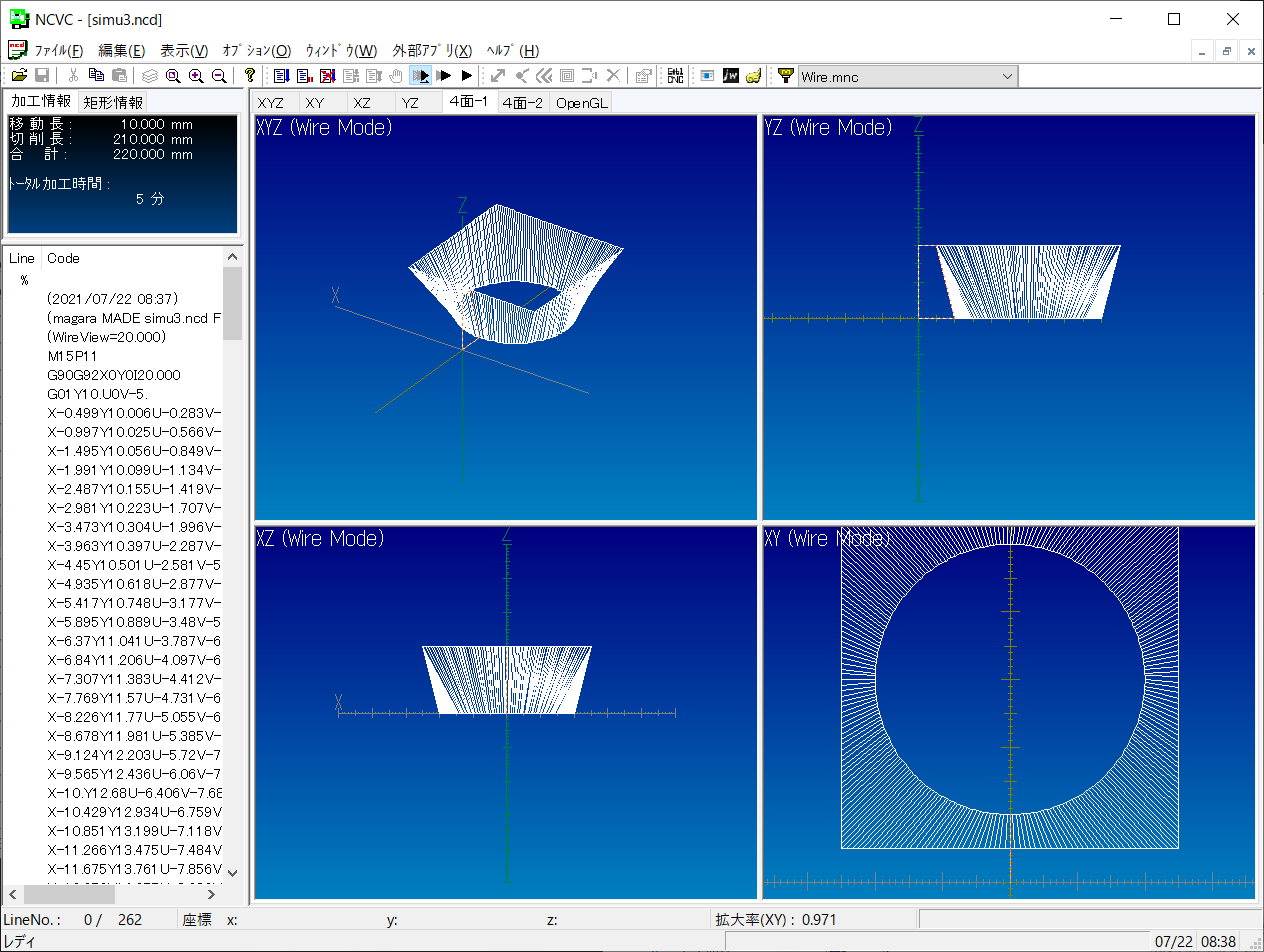
\includegraphics[scale=0.5]{No2/fig/simu3.png}
\caption{上下異形状切削のシミュレーション結果2}
\label{fig:simu3.png}
\end{figure}

 微細線分は,図\ref{fig:ncw2.png} の加工条件にある表記タブで設定します.
この場合は,円(CAM1のデータ)が先に直線補間公差で細分化され,それに合わせてCAM2(UV軸)の直線が細分化されます.
精度と加工時間を考慮して,直線補間公差を決めてください.
ただし,円の切削には若干の注意が必要です.
円データの開始位置は,0度,90度,180度,270度の4箇所だけが開始位置なので,図\ref{fig:sample4.pdf} のように角が開始位置の場合は,円を4つの円弧に分割する等の工夫が必要です.

\begin{minipage}{0.5\textwidth}
\begin{figure}[H]
\centering
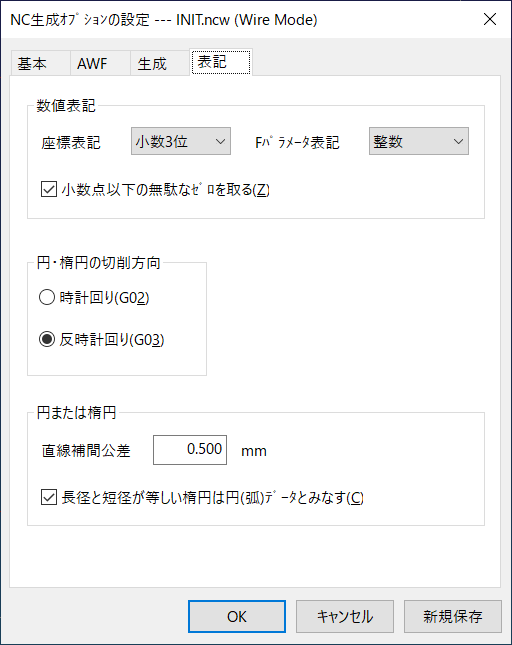
\includegraphics[scale=0.7]{No2/fig/ncw2.png}
\caption{円の直線補間}
\label{fig:ncw2.png}
\end{figure}
\end{minipage}
\begin{minipage}{0.5\textwidth}
\begin{figure}[H]
\centering
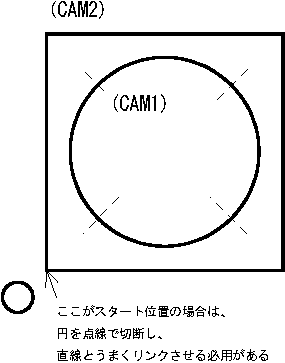
\includegraphics{No2/fig/sample4-crop.pdf}
\caption{円の分割例}
\label{fig:sample4.pdf}
\end{figure}
\end{minipage}

\subsection{上下で図形の数が違う場合 その2}
 もう1つ切削事例を見てみましょう.

\begin{figure}[H]
\centering
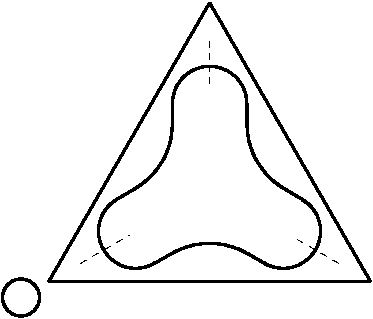
\includegraphics{No2/fig/sample5-crop.pdf}
\caption{上下異形状切削用のサンプル図形3}
\label{fig:sample5.pdf}
\end{figure}

 円弧も直線と同じく端点が開始位置なので,UV軸の図形データに均等に分割するには,点線部分で円弧を切断する必要があります.

 シミュレーション結果を図\ref{fig:simu4.png} に示します.
一部で分割幅の広い箇所がありますが,XY,UV共に直線データの場合は分割しても結果は同じはずなので自動的に調整されています.

 このように,作図時点で若干の知恵と工夫が必要ですが,XYデータとUVデータの図形が均等に割れるなら上下異形状切削データが簡単に出力できます.

\begin{figure}[H]
\centering
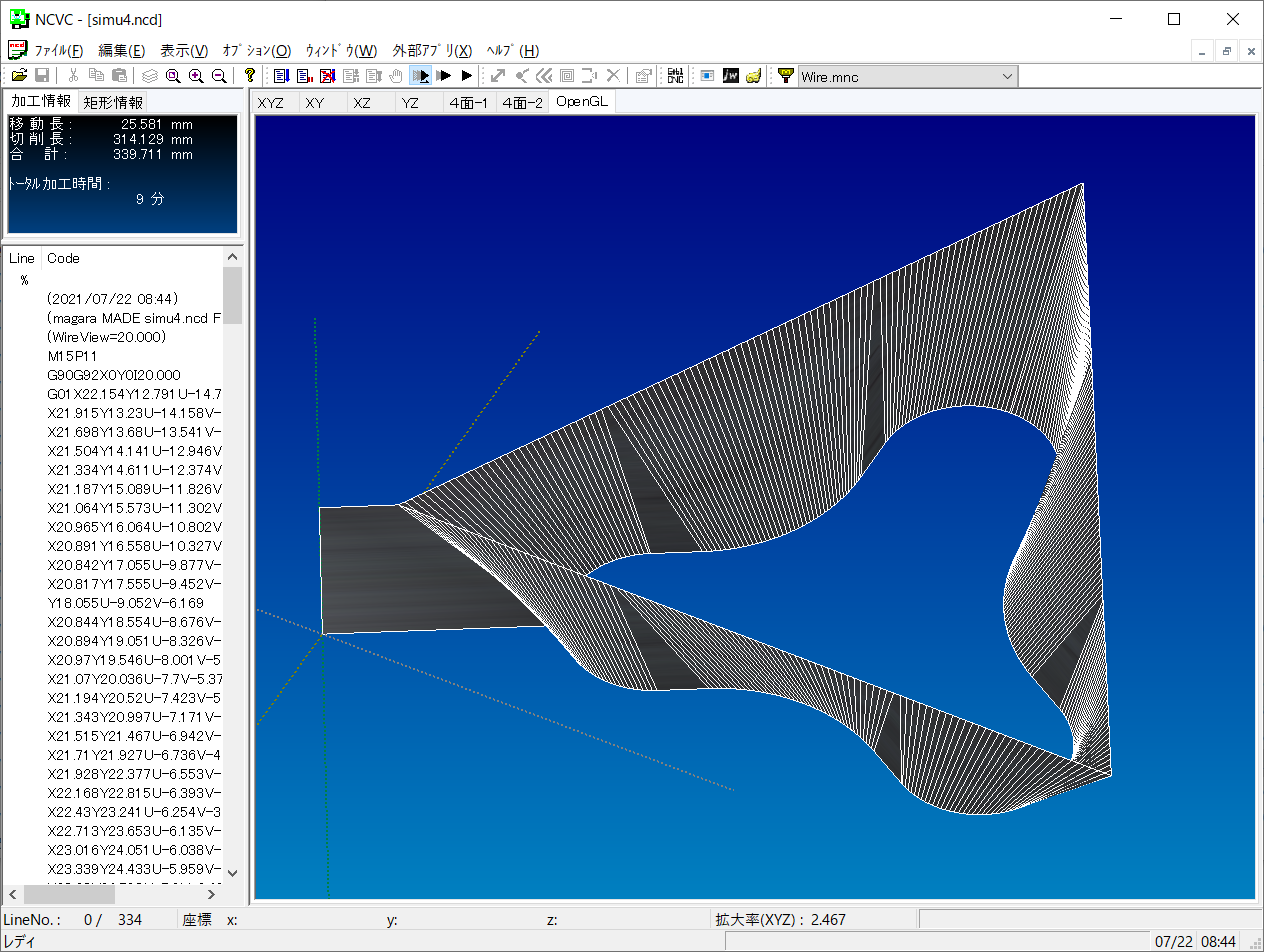
\includegraphics[scale=0.5]{No2/fig/simu4.png}
\caption{上下異形状切削のシミュレーション結果3}
\label{fig:simu4.png}
\end{figure}

\subsection{軸移動の一時停止による上下異形状切削}
 平面図形ではどうしてもXYとUVの図形オブジェクト数が合わせられない場合があります.
例えば図\ref{fig:sample6.pdf} のように外側の欠けた☆部分の線が余分で,このままではCAM1の図形データと均等割りができません.
テーパ角度の単独ブロック指令を使えば簡単ですが,NCVCではテーパ角度の単独ブロック指令は生成されません(シミュレーションはサポートされています).

\begin{figure}[H]
\centering
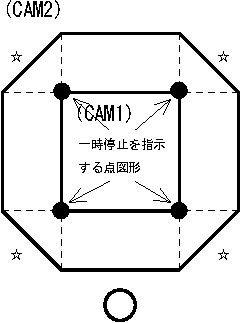
\includegraphics{No2/fig/sample6-crop.pdf}
\caption{一時停止による上下異形状切削の作図例1}
\label{fig:sample6.pdf}
\end{figure}

 ようするに,不足する側の生成を一時停止させれば良いだけで,それを指示するのが「点」の図形です(点線は補助線).
一時停止の座標で点図形を作図して生成すると,図\ref{fig:simu5.png} のように望みどおりの加工が可能です.

\begin{figure}[H]
\centering
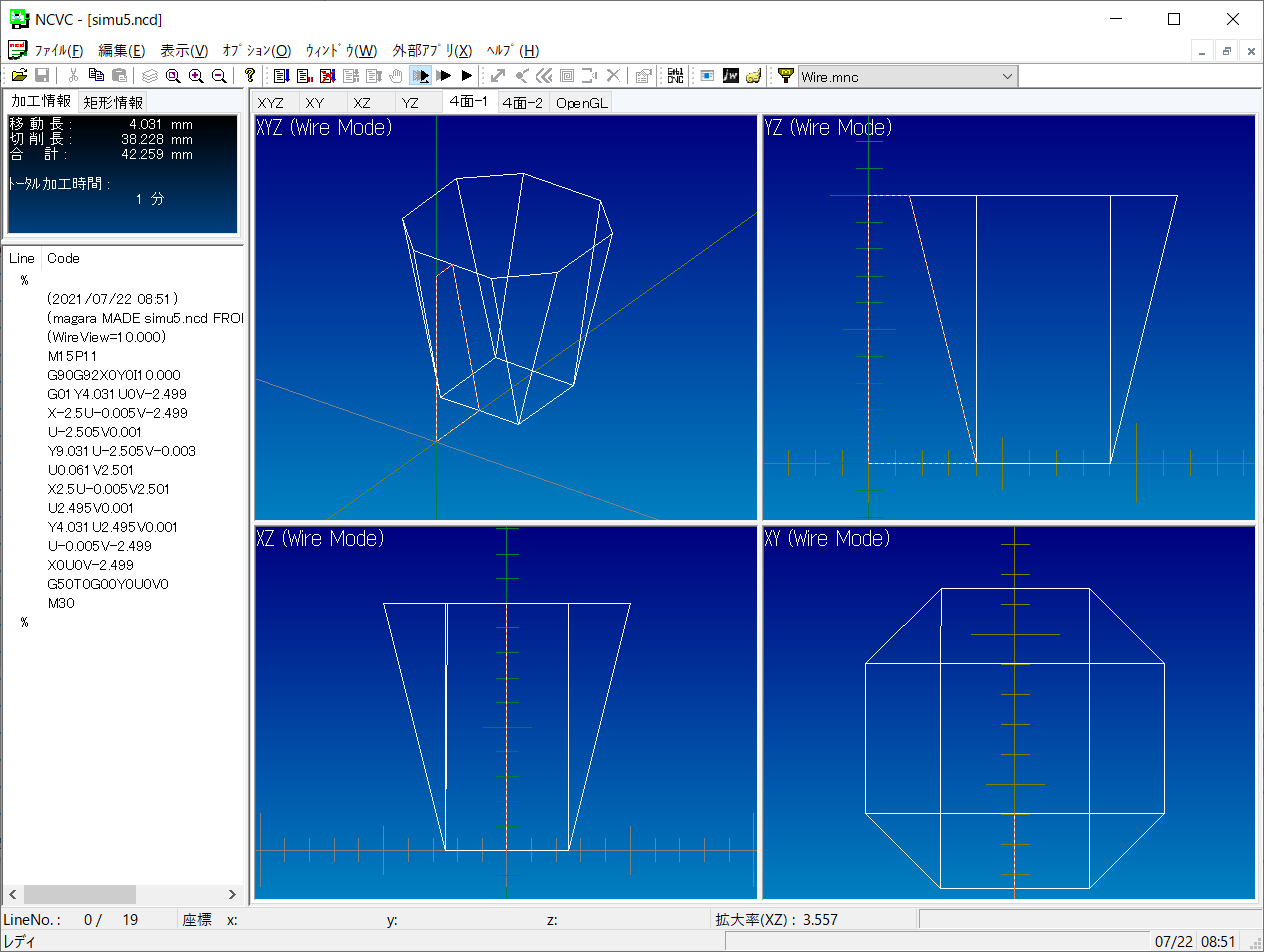
\includegraphics[scale=0.5]{No2/fig/simu5.png}
\caption{一時停止による上下異形状切削のシミュレーション結果1}
\label{fig:simu5.png}
\end{figure}

 XYとUVで過不足がなくても使えます.
例えば図\ref{fig:sample7.pdf} のようにXYデータにもUVデータにも一時停止点がある場合,
軸が交互に動きますので,図\ref{fig:simu6.png} のような加工も可能です(この場合UVデータの下辺は分割されているので,実際にはCAM2の方が線が1本多い).


\begin{figure}[H]
\centering
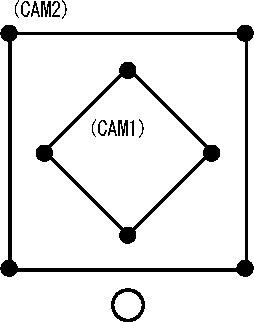
\includegraphics{No2/fig/sample7-crop.pdf}
\caption{一時停止による上下異形状切削の作図例2}
\label{fig:sample7.pdf}
\end{figure}

\begin{figure}[H]
\centering
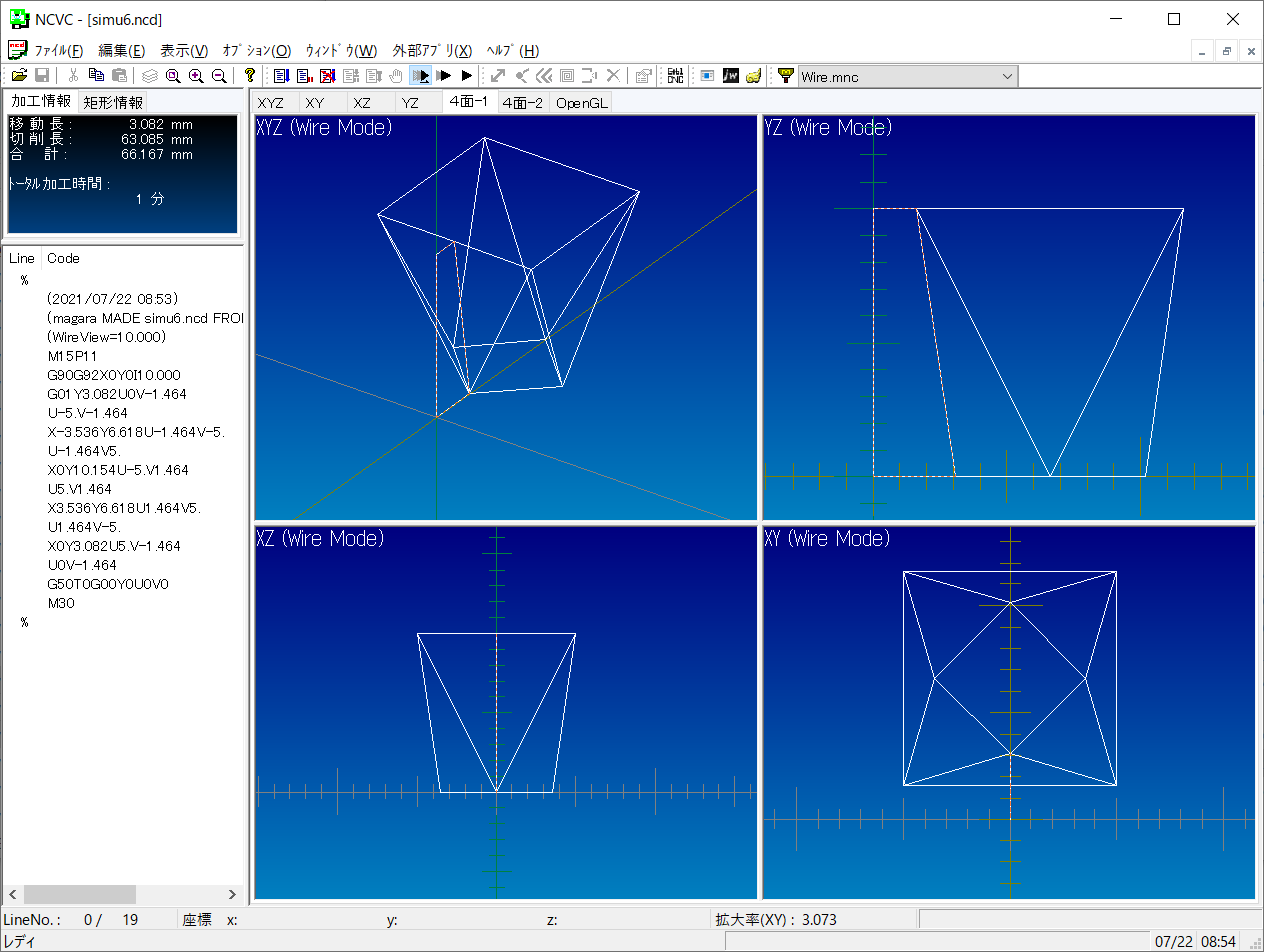
\includegraphics[scale=0.5]{No2/fig/simu6.png}
\caption{一時停止による上下異形状切削のシミュレーション結果2}
\label{fig:simu6.png}
\end{figure}

 どれもそうですが,プログラマブルな上下異形状切削はテーパ角度が機械の制限を超える場合がありますので,実際の加工前にはドライラン等で加工機でのチェックもお忘れなく.

\subsection{開始位置の意図的操作による上下異形状切削}
 最後の生成例として,はすば歯車(helical gear)のデータを生成してみます.
図\ref{fig:sample8.pdf} は見た目は平歯車ですが,サンプルとして使用するために,同じ形状を2つのレイヤに作図しています.
ホントはちゃんとひねり具合を計算して作図すべきところですが,さすが手抜き解説書!歯1枚分だけずらした「はすば歯車」を生成すると想定します.

\begin{figure}[H]
\centering
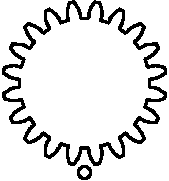
\includegraphics{No2/fig/sample8-crop.pdf}
\caption{歯車の作図例}
\label{fig:sample8.pdf}
\end{figure}

 NCVCで読ませて形状認識処理を実行します.
このサンプルでは図形が重なってわかりにくいので,\menu{表示>レイヤ}(\,\keys{Ctrl+L}\,) で他方のレイヤを非表示にし,その上で加工開始位置を設定してください.
ついでに切削方向も指示します(例では反時計回り).
そこまでの処理が図\ref{fig:start1.png} です.

\begin{figure}[H]
\centering
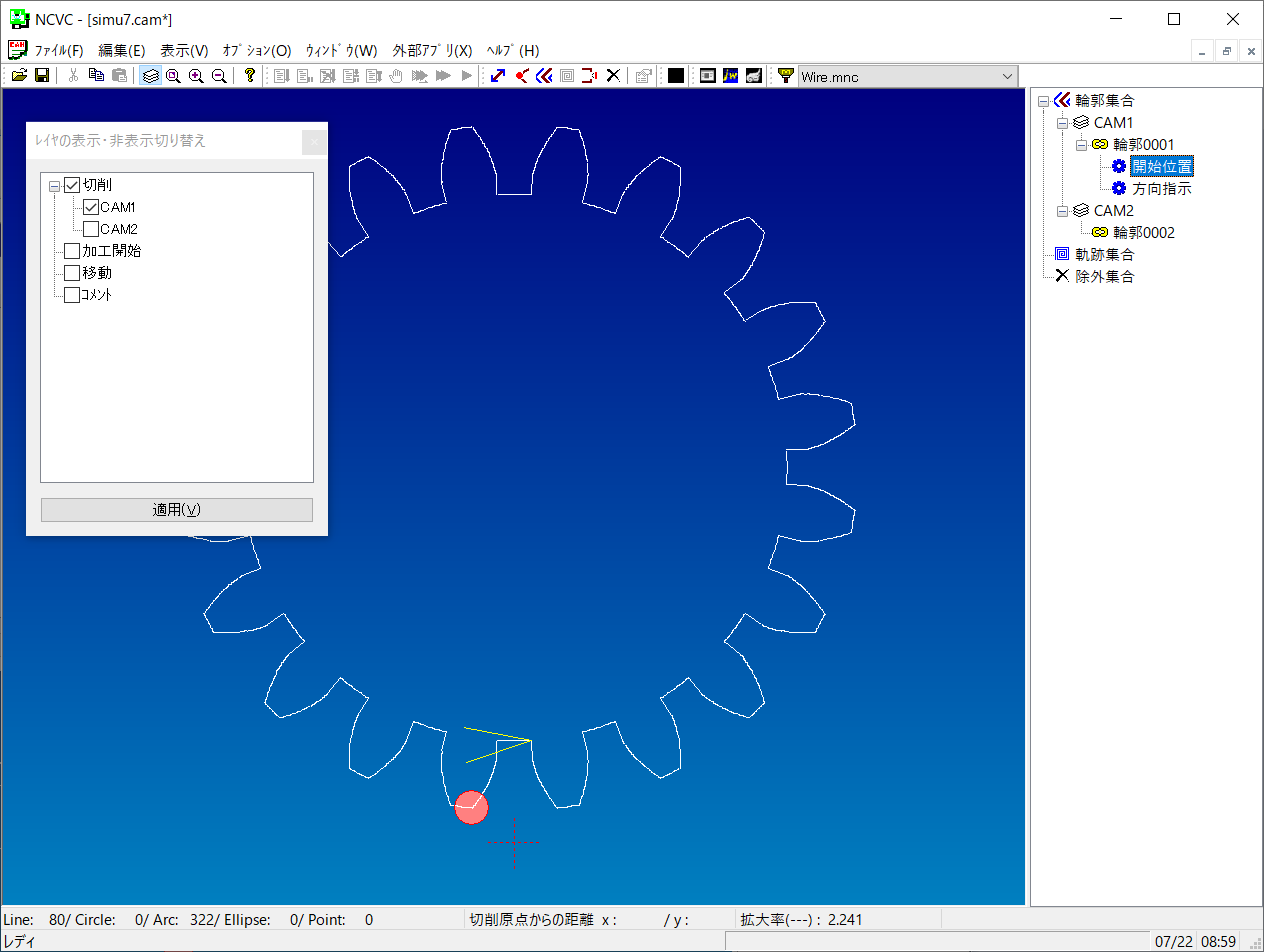
\includegraphics[scale=0.5]{No2/fig/start1.png}
\caption{加工開始位置の指示1}
\label{fig:start1.png}
\end{figure}

 次に表示レイヤを入れ替えて,同様に加工開始位置と切削方向を指示します.
歯1枚分ずれた位置を開始位置に設定してください.
何度も言いますが,あくまでもサンプルですよ(^^;).

 最終的に図\ref{fig:start2.png} のように設定してください.
切削方向は同じでもCAM1(XY),CAM2(UV)と違う加工開始位置で設定しています.

\begin{figure}[H]
\centering
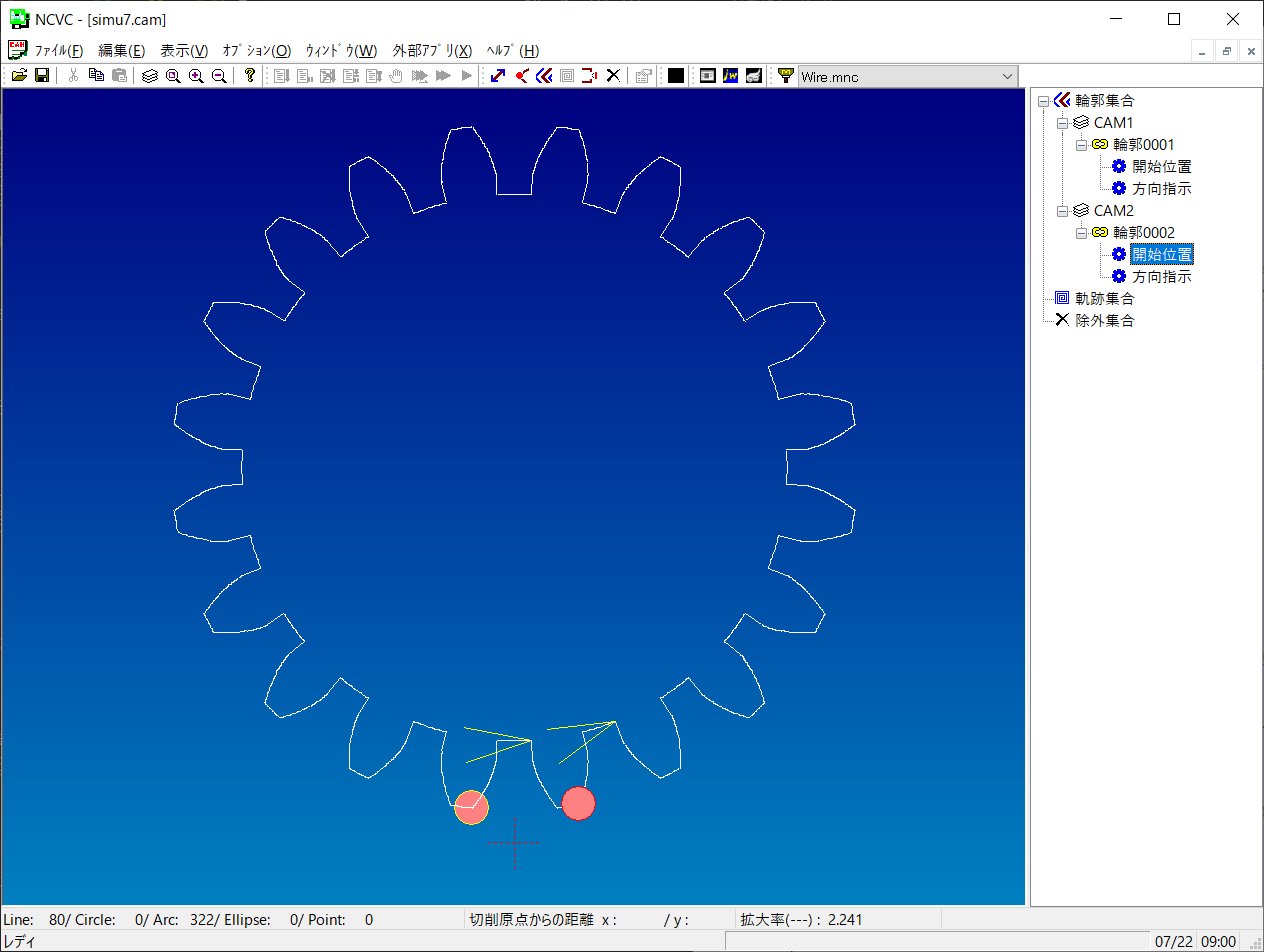
\includegraphics[scale=0.5]{No2/fig/start2.png}
\caption{加工開始位置の指示2}
\label{fig:start2.png}
\end{figure}

 これで準備OKです.
加工条件を設定し生成したシミュレーション結果が図\ref{fig:simu7.png} となります.

\begin{figure}[H]
\centering
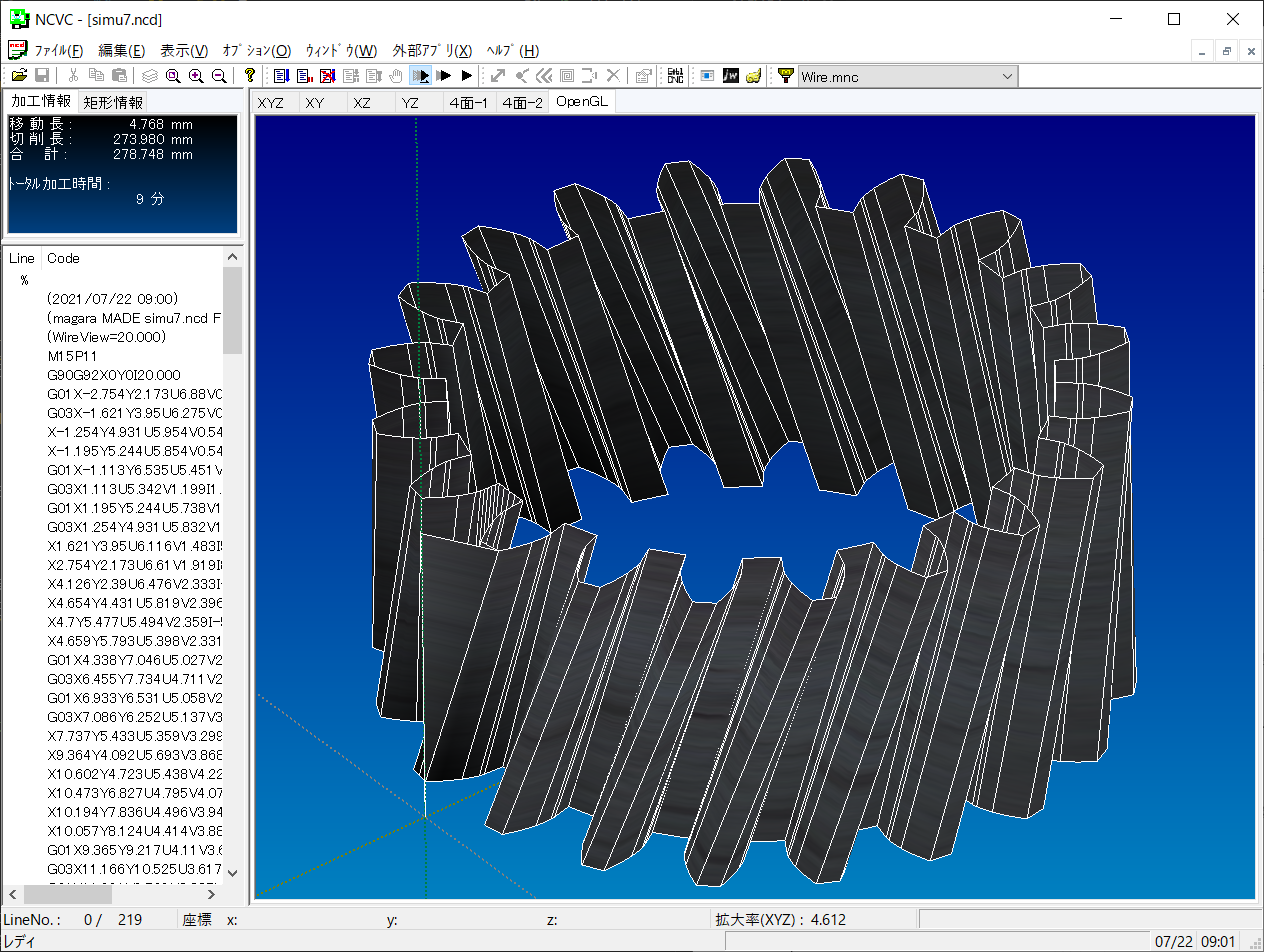
\includegraphics[scale=0.5]{No2/fig/simu7.png}
\caption{加工開始位置をずらしたシミュレーション結果}
\label{fig:simu7.png}
\end{figure}

\vspace*{3zh}
\begin{itembox}[l]{ここまでの【まとめ】}
(1) CADでの作図
\begin{itemize}
\item XY軸とUV軸の動きを2枚の切削レイヤに作図する
\item 上下の図形数を合わせる.または,均等割りできるように線切断等の処理を行う
\item 合わせられない形状は一時停止の点を作図
\item 円データは切削開始位置に注意
\end{itemize}
(2) 形状認識処理
\begin{itemize}
\item 輪郭集合に属するデータのみが対象
\item XYデータUVデータ共に必ず方向指示を行う
\item 開始位置をずらすだけでも上下異形状切削が可能
\end{itemize}
\end{itembox}
